\chapter{Vakuum}

Pro přemisťování součástek mezi zásobníkem a PDS je použita vakuová pipeta. Principielně pipeta najede nad součástku v zásobníku, zapne se odčerpávání vzduchu a součástka je nasáta na trysku. Po té přístroj s nasátou součástkou odjede na danou pozici DPS. Tam pipeta sjede v ose Z přímo nad DPS a vypne se odčerpávání – součástka se uvolní z trysky. V tomto stádiu je součástka osazena a celý proces se může opakovat.

Pro osazovací automat je základním požadavek na zdroj vakua bezolejový provoz. V případě použití bežně dostupných olejových rotačních pump hrozí riziko kontaminace součástek a DPS olejovými parami. Mohlo by tak dojít ke snížení pájitelnosti. Komerčně dostupnou variantou bezolejových – suchýh pump jsou Scrool pumpy a membránové pumpy. Jejich pořizovací cena je sice vyšší, ale odpadá problém s možnou kontaminací součástek.

\begin{figure}[h!]
  \centering
    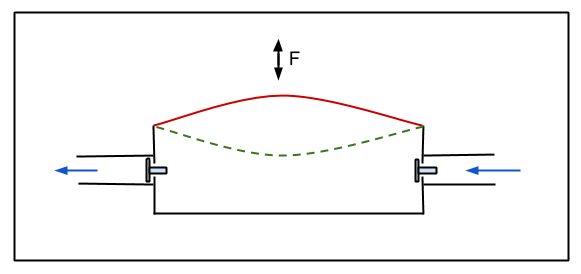
\includegraphics[width=0.6\linewidth]{obrazky/membrane.png}%
    \caption{Princip membránové pumpy.}
    \label{fig:membranka}
\end{figure}

Pro použití v osazovacím automatu byla zvolena právě membránová pumpa. Její výhodou je také minimální hlučnost. Pro srovnání u membránové pumpy Pfeiffer MVP 020-3 výrobce uvádí hlučnost (MENSINEBOROVNO) 48 dB. Rotační pumpa Pfeiffer Hena 25 se srovnatelnou čerpací rychlostí má pak hlučnost (MENSINEBOROVNO) 60 dB.

Membránová pumpa Pfeiffer MVP 020-3


Jako efektivní způsob řízení vakua se ukázalo mít pumpu neustále zapnutou a zapínání/vypínání pipety řídit pomocí ventilu. A to hlavně z důvodu čerpací rychlostí. V případě zapínání a vypínání celé pumpy by se muselo vyčerpat celé vakuové potrubí, kdežto při použití ventilů se zčerpává jen malý oběm mezi ventilem a tryskou. Celý proces je tak i za použití pumpy s nižší čerpací rychlostí dostatečně rychlý a není tak limitním faktorem pro rychlost osazování.

Z výhodou se dá mezi pumpou a ventilem použít vakuovy buffer. Pumpa ho neustále předčerpává a tvoří tak vakuovou rezervu na výkryv náhlého zvýšení tlaku po otevření ventilu. Tímto trikem se opět dosáhne mírného zrychlení k provedení jednoho cyklu.

\begin{figure}[h!]
  \centering
    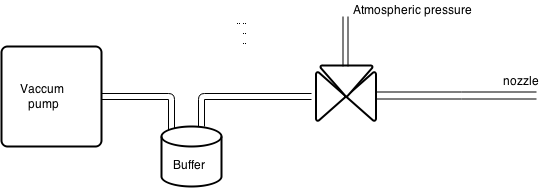
\includegraphics[width=0.8\linewidth]{obrazky/vacuum.png}%
    \caption{Uspořádání vakuové soustavy.}
    \label{fig:vacuum}
\end{figure}


S ventilem je potřeba se vypořádat s nežádoucím jevem,  že součástky v operaci umisťování na DPS zůstavají přisáty na trysce i po jeho zavření. V oblasti mezi tryskou a ventilem totiž zůstává podtlak a je proto nutné ji dostat na atmosférický tlak. To se dá řešit za pomocí druhého 'napouštěcího' ventilu, který se otevře ihned po zavření ventilu od pumpy. A nebo lépe dvoucestným ventilem. Z důvodu úspory místa a zjednodušení konstrukce jsem zvolil dvoucestný ventil. Konkrétně typ V114A-5GU od firmy SMC s napájením 24V.

\begin{figure}[h!]
  \centering
    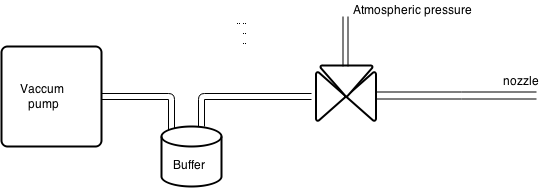
\includegraphics[width=0.3\linewidth]{obrazky/vacuum.png}%
    \caption{Vnitřní uspořádání ventilu SMC V114A.}
    \label{fig:ventil}
\end{figure}

Ventil je velice kompaktní, ale nemá možnost přímého připojení vakuového potrubí. Bylo tak nutné vyrobit rozvodný blok viz následující obrázek.  Z leva je port na připojení pipety, port uprostřed je určený na připojení tlkového senzoru. Pravý port se pak připojuje k pumpě. 

\begin{figure}[h!]
  \centering
    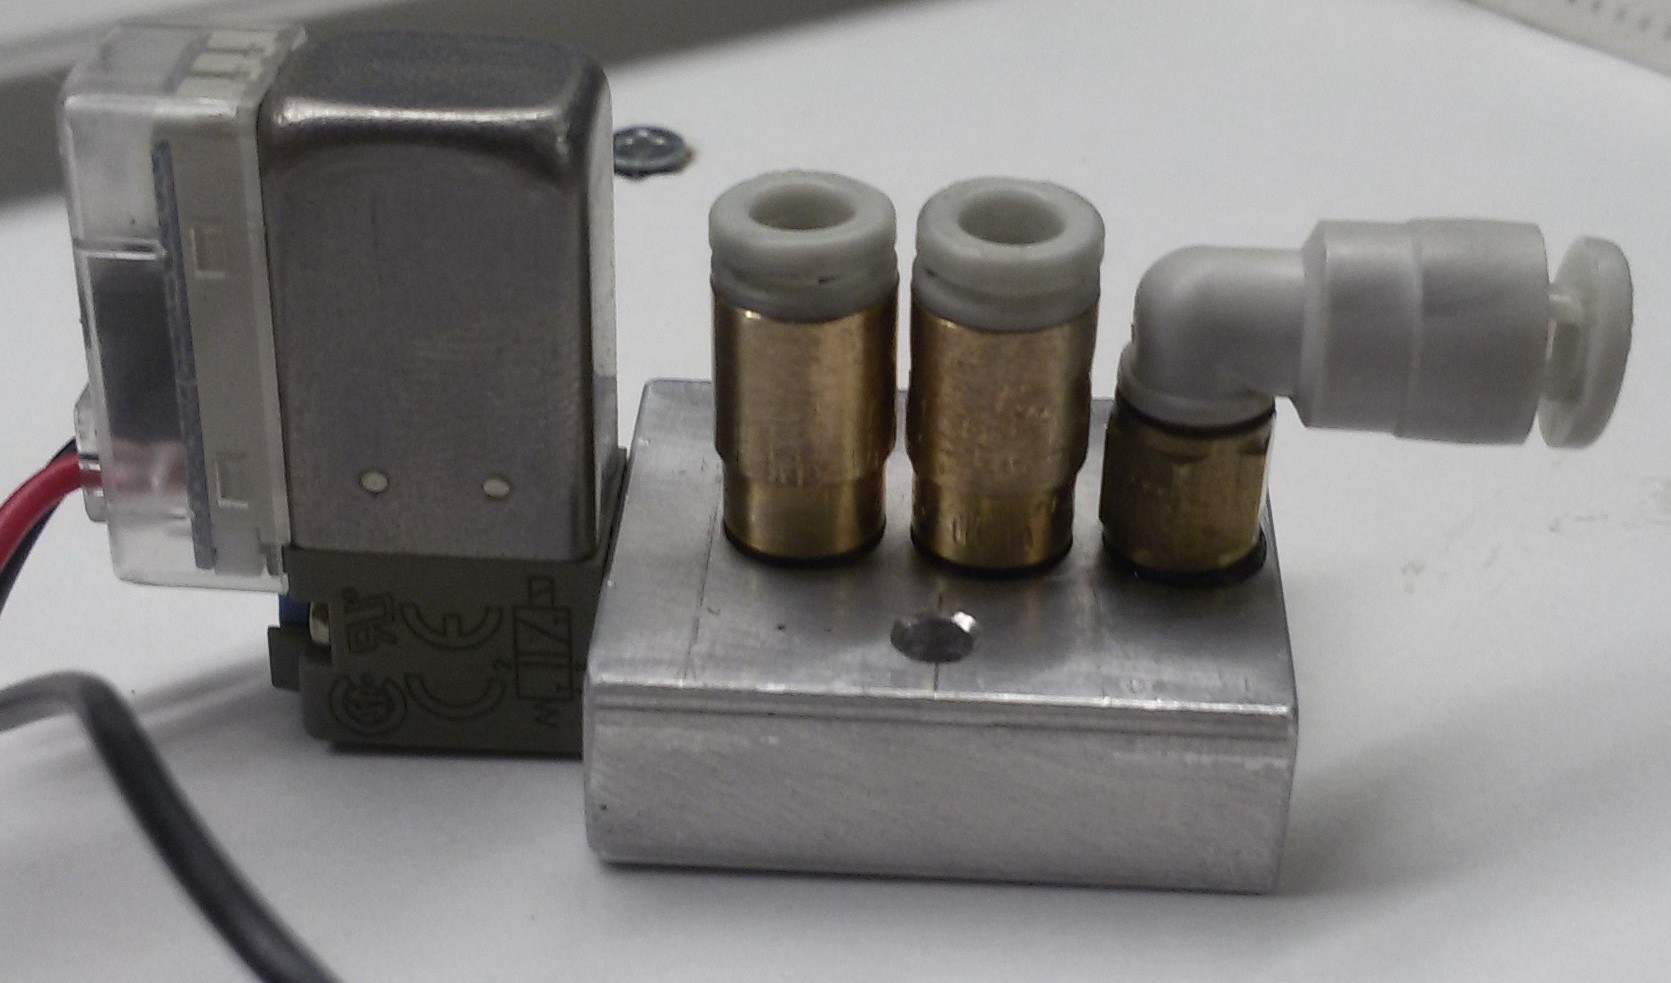
\includegraphics[width=0.7\linewidth]{obrazky/blok.jpg}%
    \caption{Rozvodný blok ventilu.}
    \label{fig:ventilblok}
\end{figure}

Vakuové porubí je z vetšiny tvořeno PTFE trubičkou s vnějším průměrem 4mm a s vnitřním 2mm. PTFE trubička je dostatešně tuhá, že u ní nedochází ke deformaci/zborcení stěn při jejím vyčeprání. Pouze na místech kde bylo potřeba malého rádiusu vedení a nebo jeho pružnosti byla použita měkčí SMC hadička z ČEHO? K připojení potrubí posloužily rychlospojeky od SMC.

Při nasávání součástek na trysku se se může stát, že se součástku nepovede nasát. Jako jeden z kontrolních mechanismů je k vakuovému potrubí připojena tlaková sodna. Pro měření vakua od atmosférického tlku až po XXX Pa se v průmyslu používají Piraniho měrky. Pro naši aplikaci ale postačí polovodičový piezorezistivní sensor v absolutní verzi. Tzn porovnávání měřeného tlaku vůči referenčnímu vakuu. 

Senzorem je potřeba detekovat následující stavy:
\begin{itemize}
\item atmosférický tlak
\item součástka přisáta na pipetě
\item součástka nepřisáta na pipetě
\end{itemize}


\begin{figure}[h!]
  \centering
    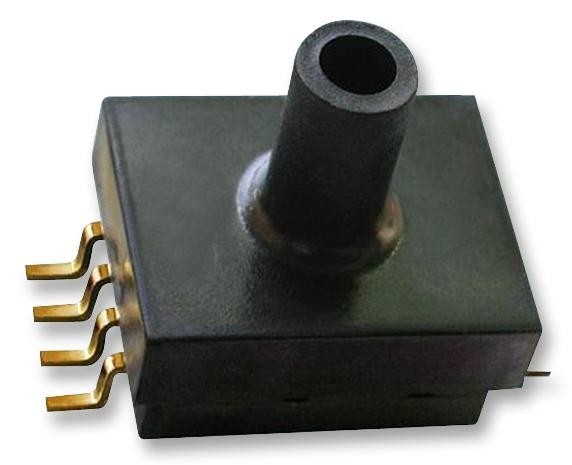
\includegraphics[width=0.4\linewidth]{obrazky/sensor.jpg}%
    \caption{Vakuový sensor  MPXM2202AS – Fotka FARNELL, nutno vyfotit vlastní.}
    \label{fig:sensor}
\end{figure}

Vybraný typ senzoru je Freescale semiconductor MPXM2202AS s rozsahem měření od 200kPa až do 0kPa.  Senzor pracuje v rozsahu napájecíh napětí 10-16V a jeho výstup je diferenciální.

Diferenciální výstup senzoru je pouhých 40mV pro celý rozsah měřených tlaků. Vybraný mikroprocesor disponuje 12 bitobvým ADC převodníkem což dává  4096 měřených úrovní. Pokud by se diferenciální napětí měřilo napřímo bez zesílení, výstup z ADC by se pohyboval pouze v rozmezí úrovní 0-50. Z toho polovina by navíc případala pro tlaky větší než atmosférické.  Rozlišení by tak bylo nedostačující.

Finální podoba  řídícího obvodu se tak skládá z lineárního stabilizítoru 7812 a diferenciálního zesilovače. Při atmosférickém tlaku byl výstup zesilovače nastaven pomocí trimru Rxxx na 3V. Se snižujícím se tlakem se výstupní napětí také snižuje.

 Senzor i s řídící elektronikou je umístěn přímo u vakuové pipety. Signálový kabel tak povede v kabelové šachtě zároveň s kabely pro Z a R motory. Z obavy, že by se na výstupním analogovém signálu mohlo indukovat rušivé napětí je řídící obvod vybaven i komparátorem, který bude mikrosprocesoru sinalizovat log 1, nebo 0 dle přítomnosti atmosféry, nebo vakua. Snahou ale bylo, aby šel analogový výstup připojit přímo na ADC mikroprocesoru.


\section{Diferenciální zesilovač - TODO}

\section{Měření výstupu z ADC}
Bylo zapotřebí vhodně zvolit odpovídající hodnoty ADC pro rozlišení jednotlivých detekovaných stavů. Proto byla provedena série měření. Předpokladem bylo, že nejhorší rozlišovací schopnost bude v případě trysky nejmenšího průměru (0,5mm), kde rozdíl v tlacích mezi stavy součástka přítomna/nepřítomna bude minimální. To se i potvrdilo, viz následující graf.

\begin{figure}[h!]
  \centering
    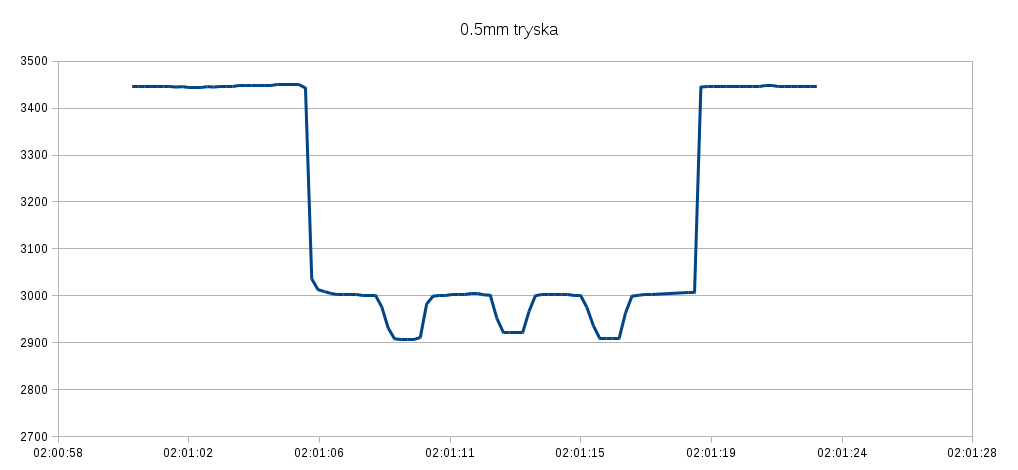
\includegraphics[width=0.9\linewidth]{obrazky/05mm_graf.png}%
    \caption{0,5mm tryska.}
    \label{fig:sensor}
\end{figure}

Rozdíl ve výstupu ADC mezi stavem součáskta přítomna/nepřítomna je přibližně 100.

Jelikož osazovací automat má výměnné trysky, byl stejný test proveden i pro trysku o průměru 0,9mm. V tomto případě byl rozdíl mezi stavy součáskta přítomna/nepřítomna mnohem markantnější – 400.

\begin{figure}[h!]
  \centering
    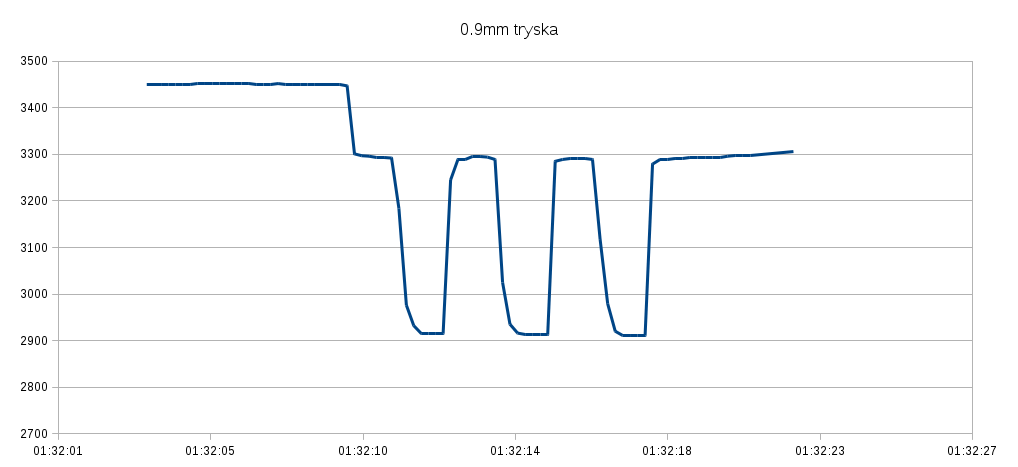
\includegraphics[width=0.9\linewidth]{obrazky/09mm_graf.png}%
    \caption{0,9mm tryska.}
    \label{fig:sensor}
\end{figure}


Rozlišovací hodnoty ADC pro jednotlivé stavy byly na základě měření stanoveny následnovně.
Atmosféra – 4096 až 3350
Součástka nepřítomna 3550 až 2950
Součástka přítomna 2950 až 0
Tyto hodnoty byly náseldně implementovýny do řídícího SW.


\section{Vakuová pipeta a tryska}
Sestava vakuové pipety musí být schopna pro vyzvednutí součástek motorizovaného pohybu v ose Z. Rozsah pohybu v ose Z je dán minimálně dvojnásobkem výšky nejvyšší osazované součástky. Dle tabulky XXX je maximální výška součástek pro 24mm pásku 11.9mm. Minimální rozsah osy tak vychází na 23.8mm. Dále je před osazením potřeba nasáté součástky na pipetě narotovat do požadované rotace. Proto musí být pipeta motorizováná i v ose R. Oba tyto požadavky komplikují vedení vakuového potrubí.

Tryska
Použití komerčně dostupné varianty trysek pro osazovací automaty nebylo pro svoji cenu a složitost adaptace uvažováno. Jako alternativa posloužily upravené injekční jehly k injekčním stříkačkám. Jehly jsou dostupné v širokém rozpětí průměrů, což je ideální pro možnost přizpůsobení velikosti trysky k dané osazované součástce. Samotnou jehlu bylo pootřeba vhodným způsobem připevnit ke hřídeli rotačního motoru. S tím také vyvstala otázka jak řešit připojení vakuového potrubí. 
Jedním z požadavků zadání diplomové práce byla možnost manuální výměny trysky/pipety. Bylo tedy zapotřebí vytvořit adaptér mezi jehlou a motorem, ke kterému se připojí vakuové potrubí.


\begin{figure}[h!]
  \centering
    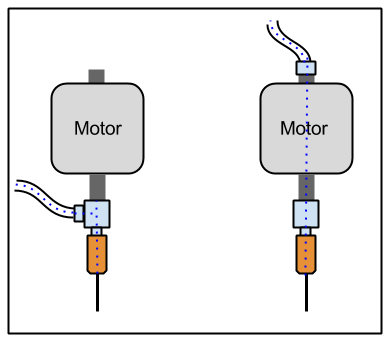
\includegraphics[width=0.6\linewidth]{obrazky/motorR.png}%
    \caption{Obrázek možných řešení vakuového vedení. Pro názornost byla modrým tečkováním naznačena cesta vakuového potrubí.}
    \label{fig:sensor}
\end{figure}

Jak ale při praktických experimentech ukázalo, tak z hlediska vyhodnocování obrazu je žádoucí mít při pohledu spodní kamerou okolo součástky uniformní pozadí. Řešení pomocí bočně připojeného potrubí tak bylo zavrženo. 
Namísto toho byl použit pro osu R motor s dutou hřídelí, která byla použita jako vakuové vedení. Toto řešení umožnilo získávat ze spodní kamery snímky s uniformním pozadím. 

Vysoustružená mosazná redukce byla k hřídeli připevněna pomocí stavěcích šroubů a zatěsněna dvousložkovým lepidlem Torrseal, který je určen do aplikací vyžadujících vakuovou těsost.
Jak zadání práce vyžadovalo, vznikla tak funkční sestava s možností manuální výměny trysky.

\begin{figure}[h!]
  \centering
    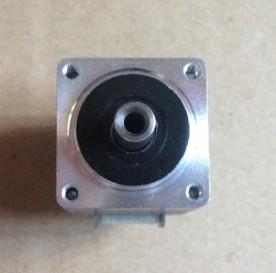
\includegraphics[width=0.6\linewidth]{obrazky/robotdigg_nema8.jpg}%
    \caption{Ukázka použitého motoru Nema8 s dutou hřídelí.}
    \label{fig:nema8}
\end{figure}

\begin{figure}[h!]
  \centering
    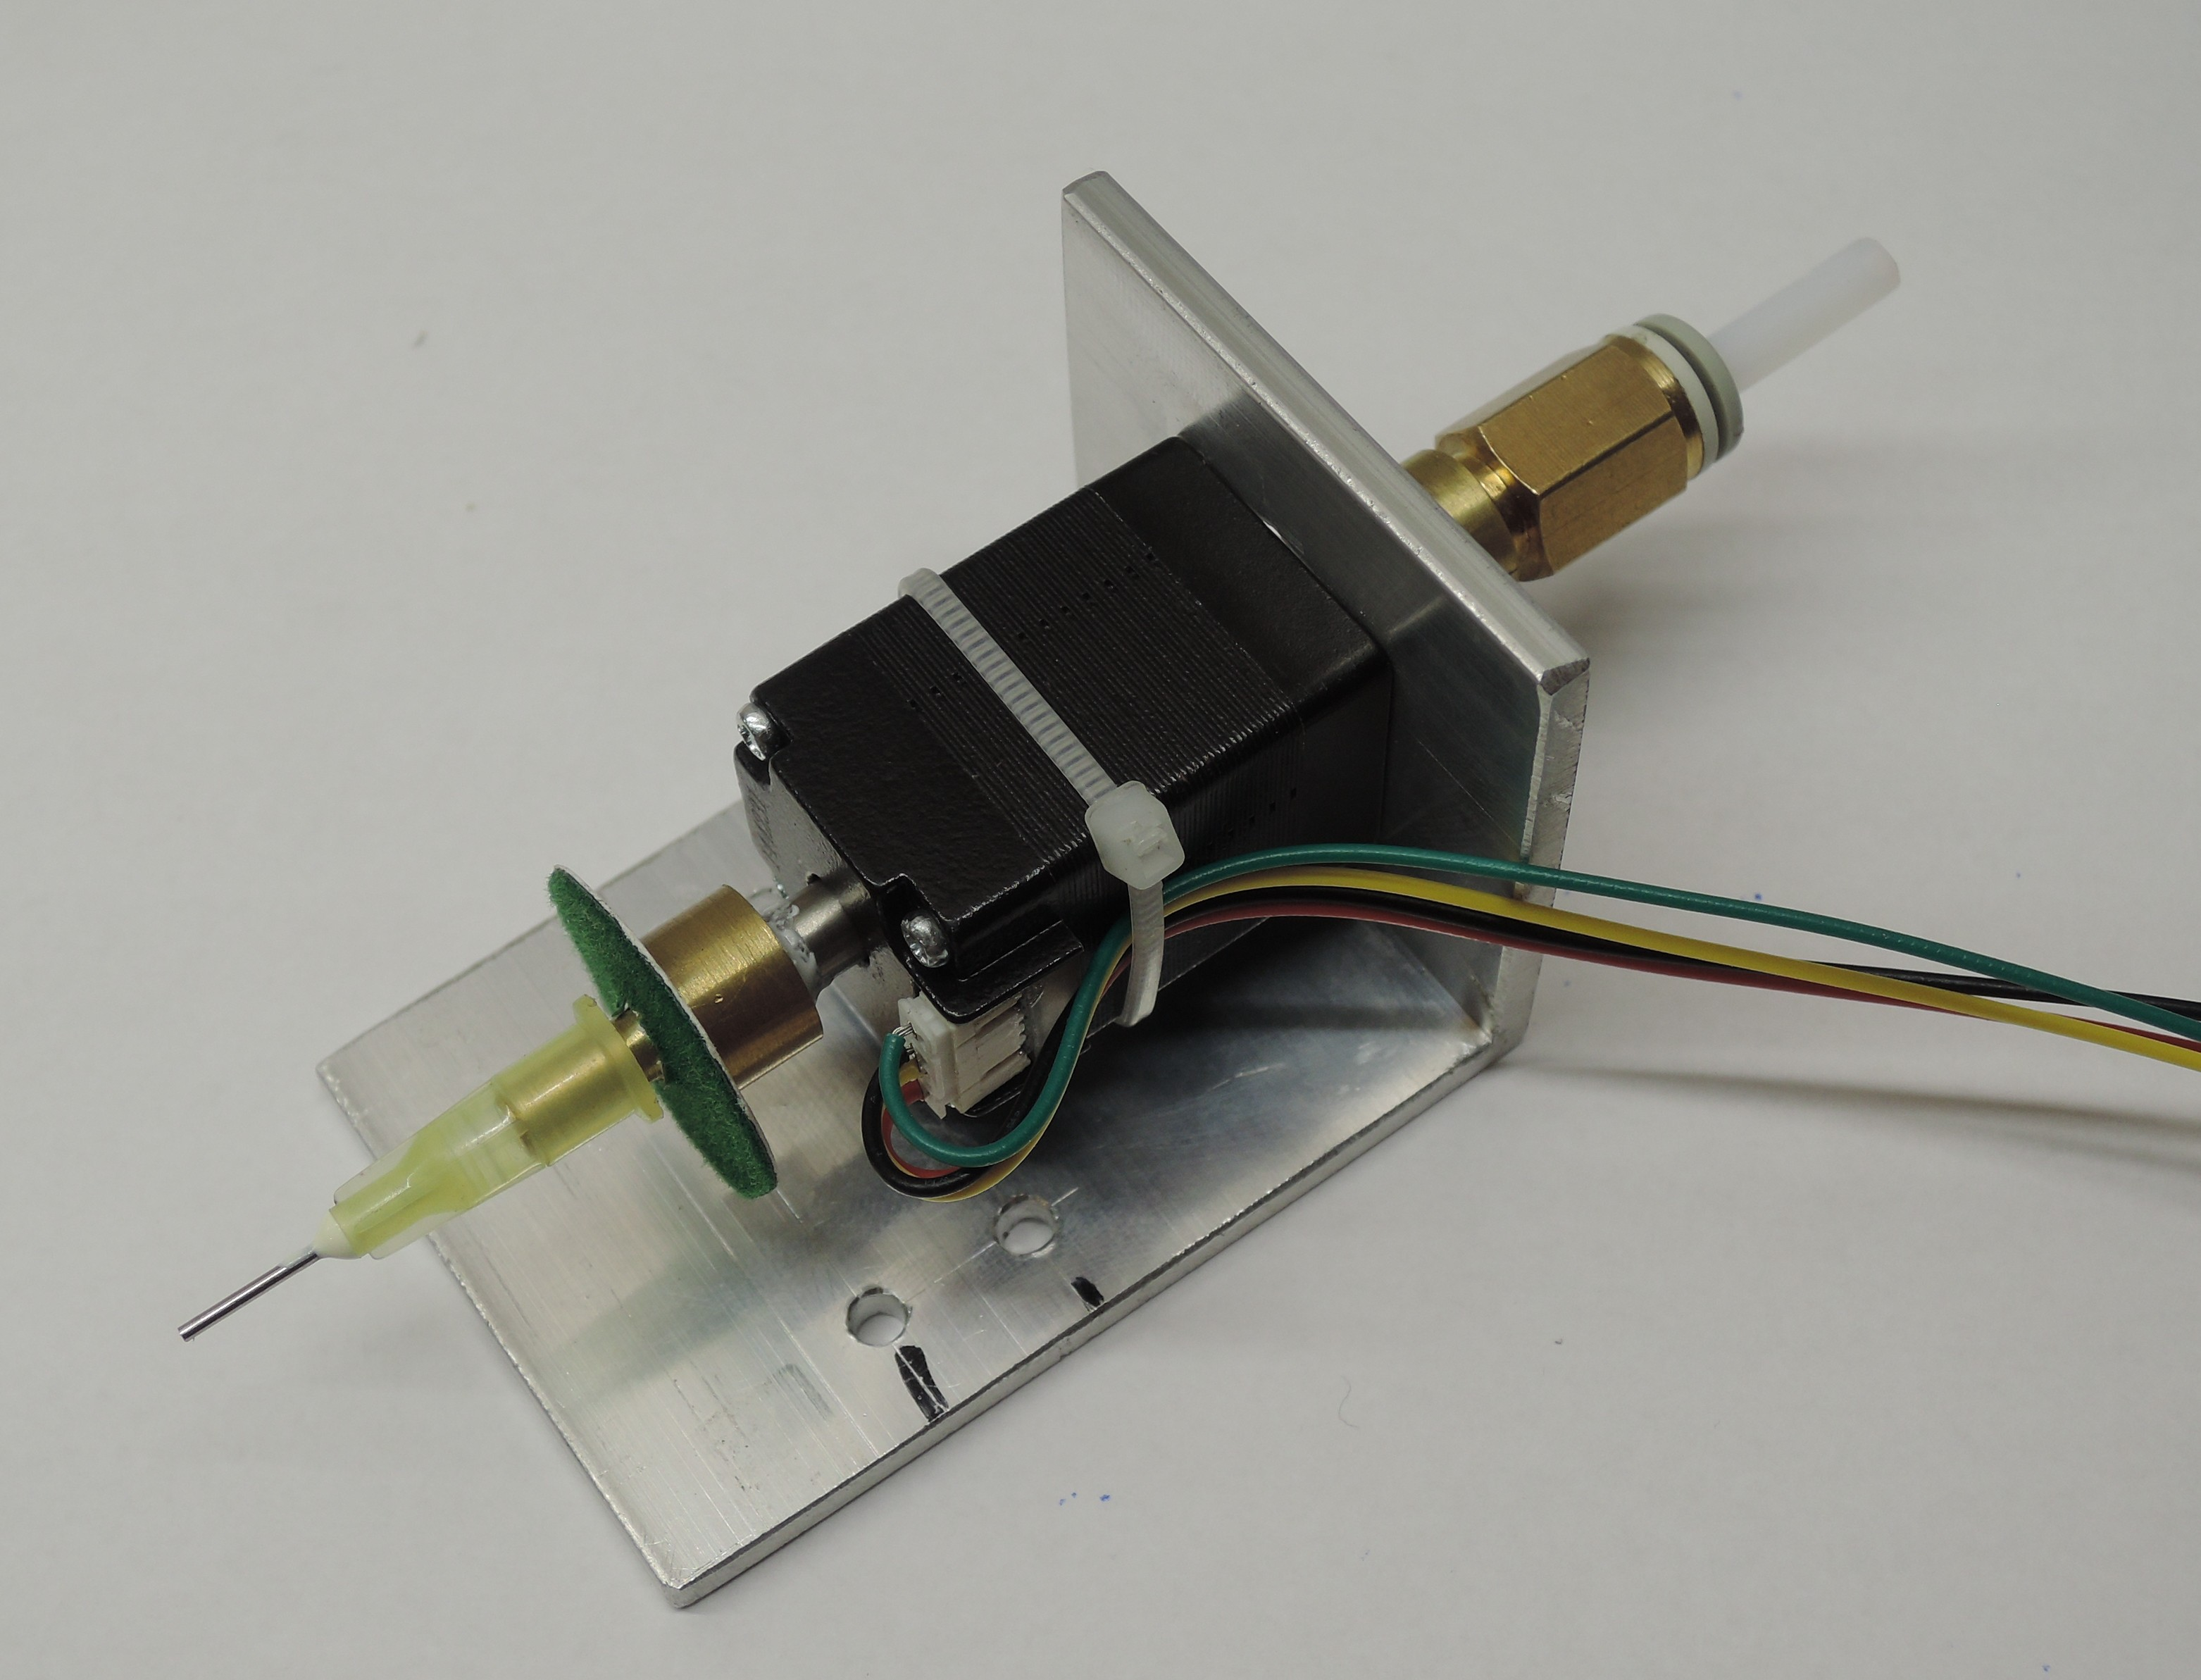
\includegraphics[width=0.8\linewidth]{obrazky/tryska2.jpg}%
    \caption{Detail vysoustružené redukce s nasazenou 0.9 mm tryskou.}
    \label{fig:tryska}
\end{figure}


